\documentclass{protokoll_en}
\newcommand{\assistent}{D. Sch�tze}
\newcommand{\versuch}{Holography}
\newcommand{\nummer}{E215}

\begin{document}

\section{Preface}

\section{Theoretical Background}
\subsection{first}
\subsection{second}
\subsection{etc}

\section{Experimentation and Analysis}
\subsection{Transmission Hologram}
To take a transmission hologram we install the set-up of figure \ref{fig:aufbau_transmiss}. It is useful to choose highly reflecting objects like silver objects.
\begin{figure}[H]
  \centering
  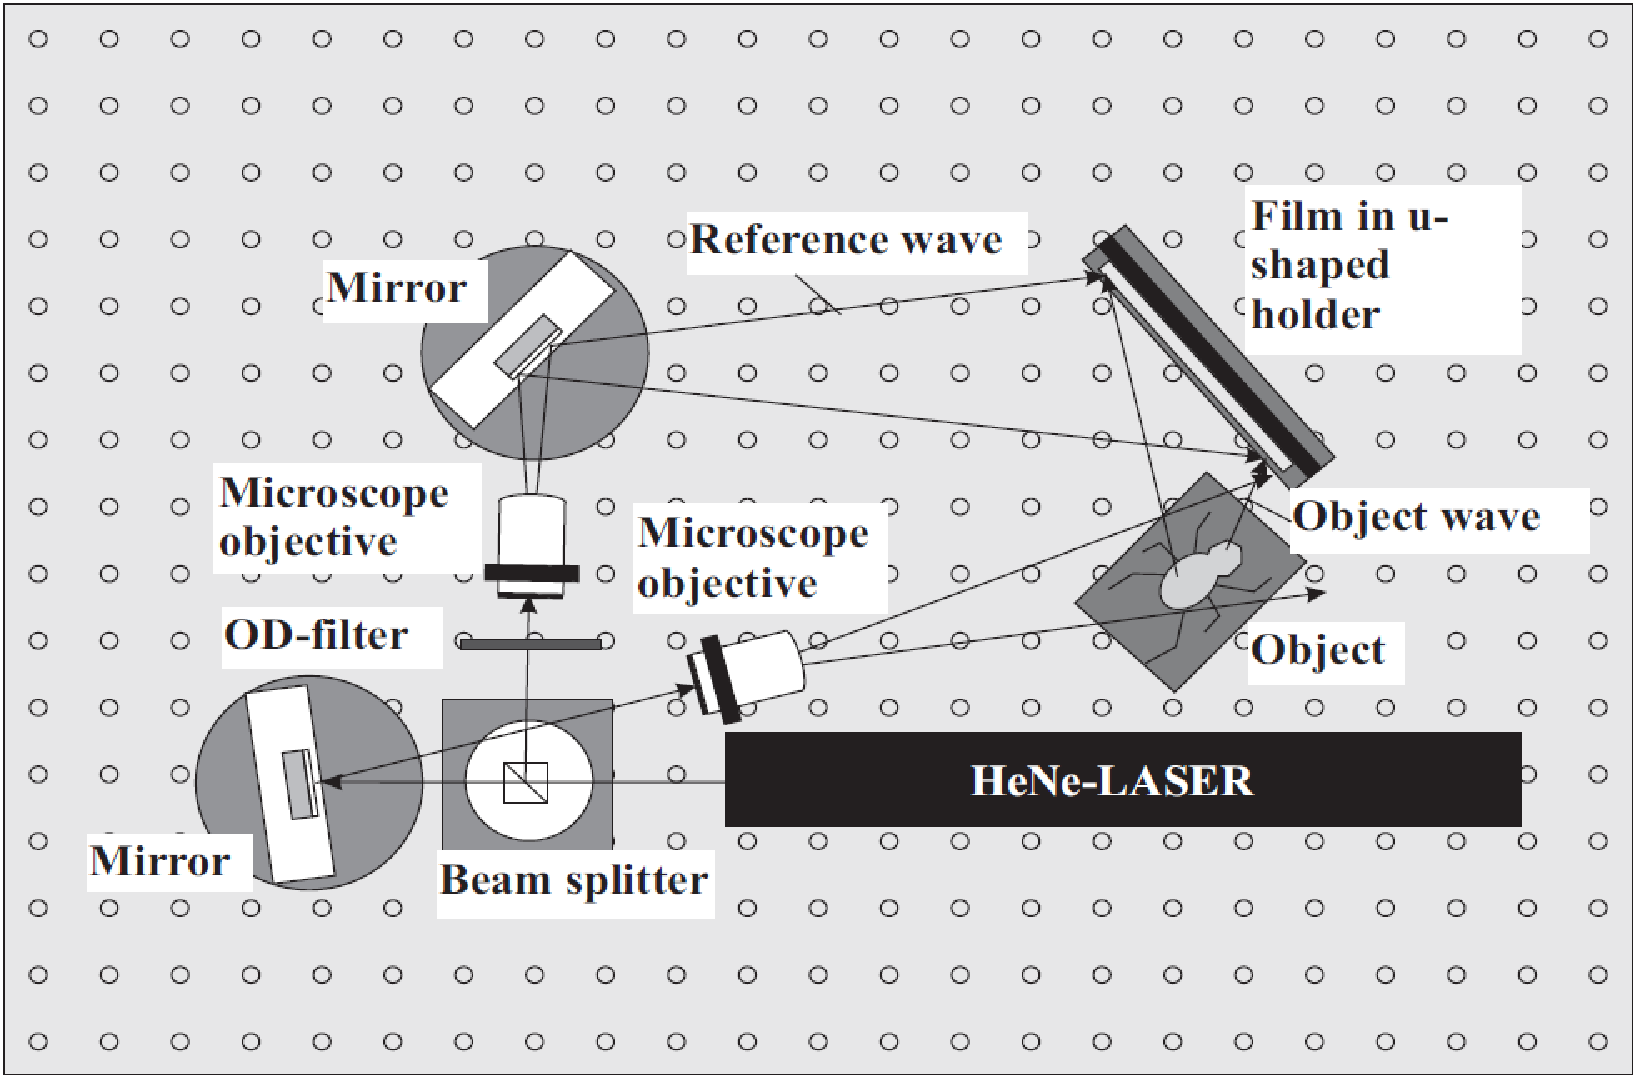
\includegraphics[width=0.5\textwidth]{graphics/aufbau_transmiss}
  \caption{Set-up for taking a transmission hologram}
  \label{fig:aufbau_transmiss}
\end{figure}
First of all one has to consider that the object and the holographic film are illuminated homogeneously. But due to reasons of coherence it is also important that the difference in pathlength of object and reference beam does not exceed approximately $\unit[30]{cm}$. Furthermore one inserts an OD filter into the reference beam to adjust the intensities of both beams. If everything is aligned properly the light is switched off except for a small LED panel and the exposure of the holographic film is done for $\unit[5]{s}$. Then the film is developed like explained in the description~\cite{skript}. For reconstruction of the object the film is placed at its position of recording, the object is removed and the object beam is blocked. Now we are indeed able to observe a three dimensional transmission hologram at the former position of the object (see figure \ref{fig:transmiss}). Unfortunately we missed to remove the OD filter while exposing the film. Therefore our hologram is weaker than it was supposed to be. Additionally the angle range for observation is rather small.
\begin{figure}[H]
    \begin{minipage}{0.2\textheight}
  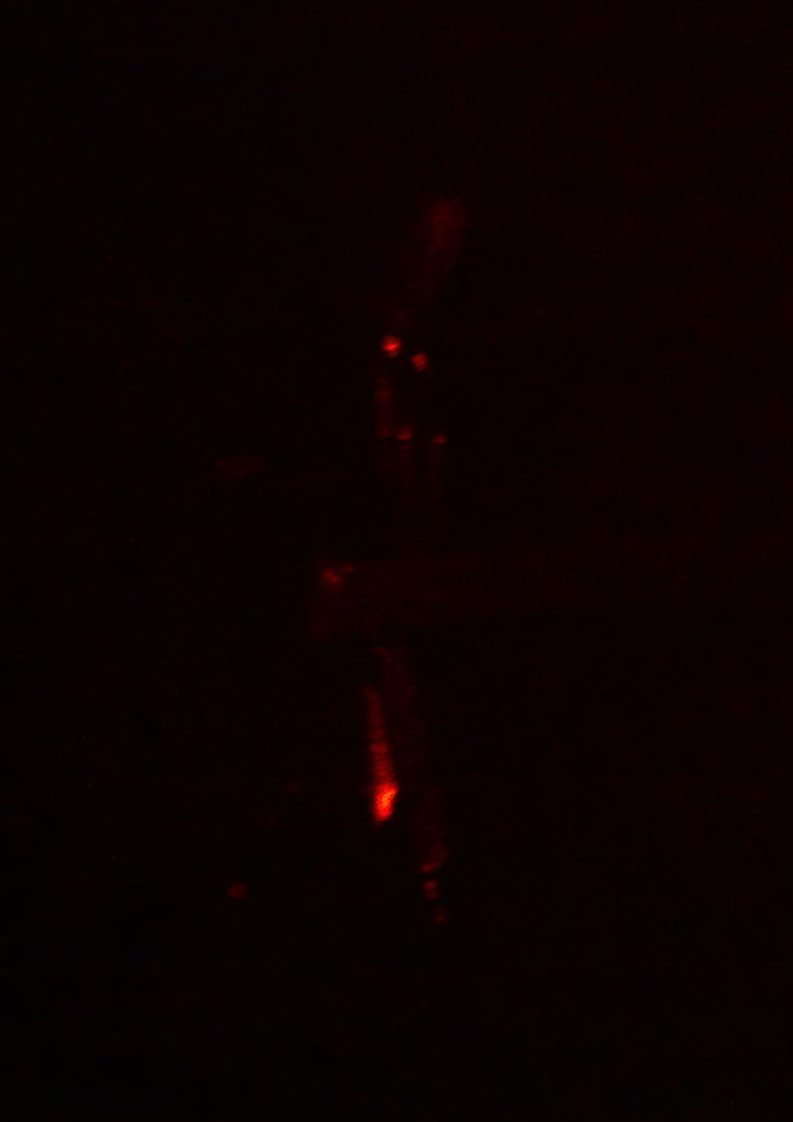
\includegraphics[width=1.0\textwidth]{graphics/transmiss1}
    \end{minipage}
    \hspace{1.3cm}
    \begin{minipage}{0.17\textheight}
  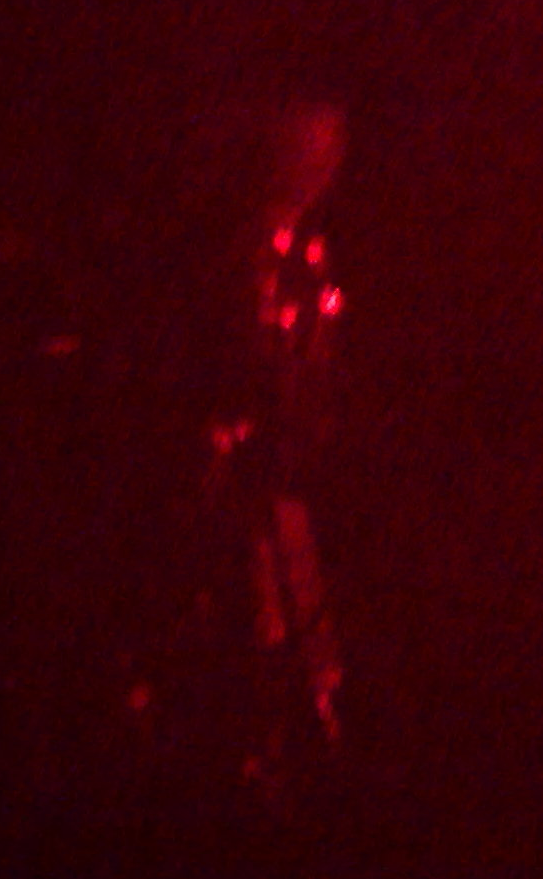
\includegraphics[width=1.0\textwidth]{graphics/transmiss2}
    \end{minipage}
  \caption{Photographs of our transmission hologram}
  \label{fig:transmiss}
\end{figure}
If one uses normal light only a spectral pattern due to the mentioned grating-like structure of the developed film is observed.

\section{Abstract}

\begin{appendix}
\section{Tables}

\Literatur{quellen}

\end{appendix}
\end{document}



